% Editable master. Rebuild the PDF and theme-aware SVG with: python3 build.py
\documentclass[10pt,tikz,border=10pt]{standalone}
\usepackage[T1]{fontenc}
\usepackage{helvet}
\usepackage{amsmath,amssymb}
\renewcommand{\familydefault}{\sfdefault}
\usetikzlibrary{arrows.meta,calc}
\definecolor{ink}{HTML}{1E293B}
\definecolor{muted}{HTML}{536277}
\definecolor{boundary}{HTML}{94A3B8}
\definecolor{oldfill}{HTML}{F3F6FA}
\definecolor{new}{HTML}{2463A8}
\definecolor{newfill}{HTML}{DCEAF5}
\definecolor{target}{HTML}{137B69}
\definecolor{targetfill}{HTML}{DDF1EC}
\begin{document}
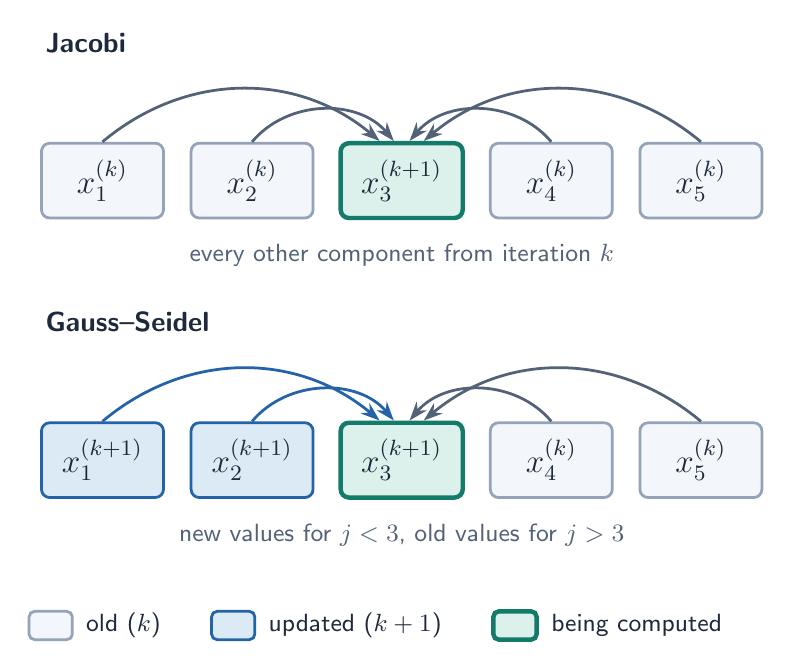
\begin{tikzpicture}[x=1cm,y=1cm,
  every node/.style={text=ink,font=\sffamily,inner sep=2pt},
  cell/.style={minimum width=1.55cm,minimum height=.95cm,line width=1pt,
    rounded corners=3pt,font=\large},
  old/.style={cell,fill=oldfill,draw=boundary},
  newer/.style={cell,fill=newfill,draw=new},
  goal/.style={cell,fill=targetfill,draw=target,line width=1.6pt},
  read/.style={-{Stealth[length=2.4mm,width=1.7mm]},line width=1pt},
  title/.style={font=\sffamily\bfseries,anchor=west},
  note/.style={font=\sffamily\small,text=muted}]

% Component row i = 3 is being computed. Cells sit 1.9 cm apart.
\def\gap{1.9}

% -------------------------------------------------------------------------
% Jacobi: every other component comes from iteration k.
% -------------------------------------------------------------------------
\begin{scope}[shift={(0,0)}]
  \node[title] at (-.8,1.75) {Jacobi};
  \node[old]  (j1) at (0*\gap,0) {$x_1^{(k)}$};
  \node[old]  (j2) at (1*\gap,0) {$x_2^{(k)}$};
  \node[goal] (j3) at (2*\gap,0) {$x_3^{(k+1)}$};
  \node[old]  (j4) at (3*\gap,0) {$x_4^{(k)}$};
  \node[old]  (j5) at (4*\gap,0) {$x_5^{(k)}$};
  \draw[read,draw=muted] (j1.north) to[out=40,in=140] ($(j3.north)+(-.28,0)$);
  \draw[read,draw=muted] (j2.north) to[out=50,in=130] ($(j3.north)+(-.10,0)$);
  \draw[read,draw=muted] (j4.north) to[out=130,in=50] ($(j3.north)+(.10,0)$);
  \draw[read,draw=muted] (j5.north) to[out=140,in=40] ($(j3.north)+(.28,0)$);
  \node[note] at (2*\gap,-.95)
    {every other component from iteration $k$};
\end{scope}

% -------------------------------------------------------------------------
% Gauss-Seidel: components above row i are already updated.
% -------------------------------------------------------------------------
\begin{scope}[shift={(0,-3.55)}]
  \node[title] at (-.8,1.75) {Gauss--Seidel};
  \node[newer] (g1) at (0*\gap,0) {$x_1^{(k+1)}$};
  \node[newer] (g2) at (1*\gap,0) {$x_2^{(k+1)}$};
  \node[goal]  (g3) at (2*\gap,0) {$x_3^{(k+1)}$};
  \node[old]   (g4) at (3*\gap,0) {$x_4^{(k)}$};
  \node[old]   (g5) at (4*\gap,0) {$x_5^{(k)}$};
  \draw[read,draw=new]   (g1.north) to[out=40,in=140] ($(g3.north)+(-.28,0)$);
  \draw[read,draw=new]   (g2.north) to[out=50,in=130] ($(g3.north)+(-.10,0)$);
  \draw[read,draw=muted] (g4.north) to[out=130,in=50] ($(g3.north)+(.10,0)$);
  \draw[read,draw=muted] (g5.north) to[out=140,in=40] ($(g3.north)+(.28,0)$);
  \node[note] at (2*\gap,-.95)
    {new values for $j<3$, old values for $j>3$};
\end{scope}

% -------------------------------------------------------------------------
% Legend.
% -------------------------------------------------------------------------
% Each item starts after the previous label, so labels cannot overlap.
\begin{scope}[shift={(-.95,-5.65)},
  swatch/.style={minimum width=.55cm,minimum height=.36cm,line width=1pt,
    rounded corners=2pt,inner sep=0pt,anchor=west},
  key/.style={font=\sffamily\small,anchor=west}]
  \node[swatch,fill=oldfill,draw=boundary] (l1) at (0,0) {};
  \node[key] (t1) at ($(l1.east)+(.08,0)$) {old ($k$)};
  \node[swatch,fill=newfill,draw=new] (l2) at ($(t1.east)+(.55,0)$) {};
  \node[key] (t2) at ($(l2.east)+(.08,0)$) {updated ($k+1$)};
  \node[swatch,fill=targetfill,draw=target,line width=1.6pt] (l3) at ($(t2.east)+(.55,0)$) {};
  \node[key] at ($(l3.east)+(.08,0)$) {being computed};
\end{scope}
\end{tikzpicture}
\end{document}
